\documentclass[a4paper,12pt]{article}
%\documentclass[aps,prl,reprint]{revtex4-1}
%\documentclass[a4paper,10pt]{extarticle}
%\documentclass[a4paper,14pt]{extarticle} 


\usepackage{cmap}  % PDF search & text copy
%% Fonts
\usepackage[utf8x]{inputenc}
\usepackage{cite}


%% Language
%	\usepackage[english, russian]{babel} % also for cyrillic, but then captions are changed to RU
\usepackage[T2A]{fontenc} % for cyrillic

%% Lines and margins
%% Double spacing
%\usepackage[nodisplayskipstretch]{setspace}
%\doublespacing  

%% Layout: choose one from below
%\usepackage[paper=a4paper,left=30mm, top=20mm, right=15mm, bottom=20mm]{geometry} 
\usepackage{fullpage} 

\usepackage{parskip} % quick setup of space between paragraphs
%\setlength{\parindent}{0pt} % no indent at the new line

%% Math
\usepackage{amsmath,amssymb,empheq}
%\numberwithin{equation}{section} % in-section equation numbering
%\usepackage{breqn}
%\usepackage{mathtools} 		%  Remove equation numbers
%\mathtoolsset{showonlyrefs} %  from unreferenced equations

%% Graphics
\usepackage{graphicx}
%\usepackage[pdftex]{graphicx}
\usepackage{caption} % graphics caption
\usepackage{subcaption}
%\usepackage{epstopdf} % include eps graphics
\usepackage{pdfpages}  % include another pdf %Usage: \includepdf[pages=-]{myfile.pdf} % \includepdf[pages={1}]{myfile.pdf}

% itemize options https://tex.stackexchange.com/a/2372
\usepackage{enumitem}
\setitemize[0]{leftmargin=10pt,itemindent=10pt} % label={-} 0 - change all levels
%\setitemize[1]{label={-}}
%\setitemize[0]{leftmargin=*}

%% \usepackage{markdown}  
% needs --shell-escape 
% use as \beging \end{markdown} - use markdown in between
% still exits with an error (because my build files are in a subfolder?)

%% PDF bookmarks
\usepackage{color,hyperref}
\definecolor{darkblue}{rgb}{0.0,0.0,0.3}
\hypersetup{colorlinks,breaklinks,
            linkcolor=darkblue,urlcolor=darkblue,
            anchorcolor=darkblue,citecolor=darkblue}

% Appendix
\usepackage[toc, page]{appendix} % toc - include in ToC; page - adds "Appendix title"

% Bibliography: test
%\usepackage{refcheck}
%\nocite{*} % Test: adds everything from .bib to bibliography

%%% COMMANDS %%%
% \newcommand* - can't connect \par; but has better error-checking
%

%% Math
\renewcommand*{\Re}{\operatorname{Re}}
\renewcommand*{\Im}{\operatorname{Im}}
\renewcommand*{\vec}[1]{\mathbf{#1}}

\newcommand*{\wt}{\widetilde} % tilde shortcut
\newcommand*{\eps}{\varepsilon}
\newcommand*{\bigO}{\mathcal{O}}

\newcommand*{\vf}{\varphi}
\newcommand*{\F}{\Phi} %{\mathbf{\Phi}}
\newcommand*{\FP}{\Phi^*}%{\mathbf{\Phi^*}} % fixpoint 

\newcommand*{\D}{\Delta}%{\mathbf{\Delta}} % Delta0
\newcommand*{\Lmap}{\mathcal{L}} % Poincare map
\newcommand*{\Lmat}{\mathbf{L}}  % Linearized Poincare map

%% Bibliography
\newcommand*{\doi}[1]{\href{http://dx.doi.org/#1}{doi: #1}}

\begin{document}

\setcounter{secnumdepth}{0} % sections dont get numbered
%\setcounter{tocdepth}{1} % Show sections
\setcounter{tocdepth}{2} % + subsections
%\setcounter{tocdepth}{3} % + subsubsections
%\setcounter{tocdepth}{4} % + paragraphs
%\setcounter{tocdepth}{5} % + subparagraphs

\tableofcontents

\clearpage



\section{Notation}

\begin{itemize}
\item $\mathbf{k}$ - wave vector, $[\frac{\text{rad}}{\mu\text{m}}]$. 
\item $k_1$, $k_2$ - wavenumber\footnote{In wikipedia and a number of papers the wave number is the same as the wave vector, but in 1D. It has dimensions of $\frac{\text{rad}}{\mu\text{m}}$ rather than being dimensionless integer. But in \cite{zou2009} authors use the same definition of the wave number as we do.}
\item ($k_1$,$k_2$)-twist, $\vec{k}$-twist, splay state \cite{strogatz1993}
		
\item $\mathbf{\Phi}= (\varphi_1, \varphi_2, .., \varphi_{N})^T $ - phase vector
\item $ \mathbf{Q(\Phi)}$ - vector of active driving forces
\item $ \mathbf{\Gamma}$ - friction coefficients NxN-matrix
\item $\mathbf{\Phi_k}$ - m-twist solution
\item $\phi(\mathbf{\Phi})$ - global phase, according to one of the definitions. 

	\textit{Currently mean phase is the default choice for global phase.}
\item $\mathcal{L}: H \rightarrow H$ - Poincare map
\item $\mathbf{\Phi^*} \in H$ - fix point of the Poincare map
\item $\mathbf{\Phi^{*}_k}$ - fix point close to the m-twist solution
\item $\mathbf{\Delta_0}$, $\mathbf{\Delta_1}$ - perturbation initial and after one cycle: $\mathcal{L}(\mathbf{\Phi^{*}} + \mathbf{\Delta_0}) = \mathbf{\Phi^{*}} + \mathbf{\Delta_1}$
\item $\mathbf{L} = \mathrm{D}\mathcal{L}(\mathbf{\Phi^*})$ linearized Poincare map at a fixed point (matrix). In code `Lmat`
\item $\Lambda_j$ - eigenvalues of $\Lmat$, Floquet multipliers
\item $? = \ln \Lmat $  logarithm of the linearized Poincare map. In code `Lmat\_log`
\item $\lambda_j$ - eigenvalues of $\ln \mathbf{L}$, dimensionless Lyapunov exponents
\end{itemize}

\subsection{Conflicts}

\begin{itemize}

\item Fixpoint notation and complex conjugation.
\item Once $\delta$ and $\D$ are taken - how to denote a difference of some values? -> use $v$ for eigenvector?
\item global phase and components of $\mathbf{\Phi}$: set global phase to $\phi$ instead of $\varphi$?
\end{itemize}


\section{Geometry}

*Unit vectors*
$$
\mathbf{e}_1 =\left( \begin{array}{c} 1 \\ 0 \end{array} \right), \quad
\mathbf{e}_2 =\left( \begin{array}{c} \frac{1}{2} \\  \frac{\sqrt{3}}{2} \end{array} \right).
$$

Position vectors
$$
\mathbf{x}_{n,m} = n\,a\,\mathbf{e}_1 +  m\,a\,\mathbf{e}_2
$$

Honeycomb lattice
$$
\mathcal{H} = \{ \mathbf{x}_{n,m} | 2n+m \equiv 0 \text{ or } 2 \text{ mod } 3\}
$$

Triangular lattice
$$
\mathcal{T} = \{ \mathbf{x}_{n,m} | n,m \in \mathrm{Z} \}
$$

\section{m-twist solutions}

Wave vector of metachronal wave consistent with periodic boundary condition
$$ \mathbf{k} = \frac{a_1}{L_1}\,k_1\,\mathbf{a}_1^* + \frac{a_2}{L_2}\,k_2\,\mathbf{a}_2^*, $$
where $k_1,k_2\in{Z}$ and $a_1=a$, $a_2 = \sqrt{3} a/2$

Meta-chronal wave solutions:

Phase-space vector
$ \Phi (t) = (\varphi_1, \varphi_2, .., \varphi_{N})^T $
with components
$$
\varphi_j(t) = \varphi(t) - \mathbf{k} \cdot \mathbf{x}_j,
$$
for some global phase $\varphi(t)$.
We expect $\dot{\varphi}\approx\omega_0$, but only approximately, since the calibration of active driving forces does not take into account the (weak) hydrodynamic interactions.

\subsection{Dynamic equation from force-balance equation}

We start with
$$  \mathbf{\Gamma}(\Phi) \dot{\Phi} =Q(\Phi),$$
or
\begin{equation}
\dot{\Phi} = \mathbf{\Gamma}^{-1}(\Phi)Q(\Phi) 
\label{eqn:phi_gamma}
\end{equation}


This linear system can be solved directly in Python.

We calibrate dynamical simulations with pair-wise coupling functions from hydrodynamical simulations
$$ \Gamma_{ij}(\Phi) = 0 \quad \text{if not neighbours} $$
$$ \Gamma_{ij}(\Phi) = \Gamma_{12}^{\mathrm{(loc)}}(\varphi_i,\varphi_j; a, \psi) \quad \text{if neighbours} $$
where the translation vector pointing from cilium $i$ to cilium $j$ reads
$$[n(j)-n(i)]\,\mathbf{e}_1 + [m(j)-m(i)]\,\mathbf{e}_2 = a \left( \begin{array}{c} \sin\psi \\ \cos\psi \end{array} \right).$$

Self-friction:
$$ \Gamma_{ii}(\Phi) = \Gamma_{11}^{\mathrm{(loc)}}(\varphi_i, \varphi_j; a, \psi) $$

Note, self-friction $\Gamma_{11}^{\mathrm{(loc)}}(\varphi_i, \varphi_j; a, \psi) $ dependence on $\varphi_j$, $a$, $\psi$ is so weak\footnote{assuming $a$ is big enough}, that we can take
$\Gamma_{11}^{\mathrm{(loc)}}(\varphi_i, \varphi_j; a, \psi)= \Gamma_{11}^{\mathrm{(loc)}}(\varphi_i)$

We therefore calibrate active driving forces as following
$$ Q_{i}(\Phi) = \Gamma_{11}^{\mathrm{(loc)}}(\varphi_i) \omega_0 $$


\subsection{Global Phase}

\subsubsection{Naive phase}
For some index $j$, $\phi = \mathbf{\varphi}_j$

\subsubsection{Circular average phase}

We define order parameters
\footnote{[Kuramoto, 1984](https://link.springer.com/chapter/10.1007/978-3-642-69689-3\_7)  [[Strogatz, 2000]](https://www.sciencedirect.com/science/article/pii/S0167278900000944)}
\footnote{Notation $r$ - from [Schröder, Timme - univ. order parameter arXiv:1704.04130v1]}
for each metachronal wave vector $\mathbf{k}$

$$r_\vec{k}(\F) = \left| \frac{1}{N}\sum_j \exp\left[ i ( \varphi_j - \varphi_{\vec{k},j} ) \right] \right|,$$

where $\varphi_{\vec{k},j}$ - j-th component of $\Phi_\vec{k}$, m-twist solution defined by vector $\vec{k}$.

Then, for a fixed $\vec{k}$ we can define a global phase:
$$\phi_{\vec{k}}(\F) = \arg \left( \frac{1}{N}\sum_j \exp\left[ i ( \varphi_j(t) - \varphi_{\vec{k},j} ) \right] \right) $$

Unfortunately, this definition is only meaningful when $S_\vec{k}$ is close to 1.

\subsubsection{Mean phase}

Define the global phase as algebraic mean of all phases
$$
\phi =  \frac{1}{N}\sum_{j=1}^{N} \varphi_j
$$

Pros
\begin{itemize}

\item Additive: if $\mathbf{\Phi} = \mathbf{\F_0}+ \mathbf{\F_1} $, then $\phi(\F) = \phi(\F_0) + \phi(\F_1)$
\item As an implication, it is independent of which initial condition we consider.
\item Poincare surface will be a plane, defined by normal $(1,1,1,1..,1)$.

  [A language of quotient vector space could be useful; just keep this reference here for now http://mathworld.wolfram.com/QuotientVectorSpace.html]
  (quotient = частное)

\end{itemize}

Cons
\begin{itemize}
\item $\varphi_j$ can't jump from  $2 \pi$ to $0$, otherwise the global phase will make a jump by $- \frac{2 \pi}{N}$.
\end{itemize}


\section{Poicnare map for an m-twist solution}
\subsection{Poincare map and limit cycle}
We consider a Poincare section $H$ defined by

$$
H =\{ \Phi : \varphi(\Phi) \equiv \varphi(\Phi_0) \mod 2\pi \}.
$$
where $\varphi$ denotes the global phase, $\Phi_0$ is the phase vector at initial time $t_0$. 

 $H$ is a $(N-1)$-dimensional hyper-surface in $N$-dimensional phase space. If $\varphi$ is the mean phase, $H$ is a hyperplane.

For each of m-twists solutions, we anticipate a corresponding limit cycle $C_\vec{k}$, piercing $H$ close to $\Phi_k$ i.e.

$$
C_\vec{k} \cap H_0 = \Phi_\vec{k} + \mathbf{E}^*,
$$

with a small correction vector $\mathbf{E}^*$.
The reason for the small correction $\mathbf{E}^*$ is that the calibration of active driving forces causes small phase-dependent variations of the instantaneous phase speed \textit{(a cilium will speed up at one part of the beat cycle, and slow down at another; but then the phase difference will vary during the cycle, therefore we don't get a perfect m-twist, which has constant phase difference?)}.

Therefore, the first step is to find $\Phi^*_\vec{k}=\Phi_\vec{k} + \mathbf{E}^*$.

We define the \textbf{Poincare map} $\mathcal{L}: H \rightarrow H$ as
 $$\mathcal{L}(\Phi_0) = \Phi_1,$$
where
$\Phi_0 = \Phi(t_0)$ - some initial phase\footnote{Note that for any $\Phi_0$ we can define a Poincare section as defined above.},
$\Phi_1=\Phi(t_1)$ - where $t_1$ is the next time when our phase trajectory intersects with the Poincare section.

With this definition  $\Phi^*_\vec{k}$ is a fixed point of Poincare map.

\textit{TODO: explain why it cannot be another limit cycle in Poincare plane. }

\textit{TODO: do we expect no extra fixed points/ limit cycles?}

\subsubsection{Procedure to find the fixpoint $\Phi^*$}

By definition, the fixpoint is such a point that
$$
\mathcal{L}(\Phi^*) = \Phi^*
$$
We define
$$
D(\Phi) = \mathcal{L}(\Phi) - \Phi
$$
and
$$
d(\Phi) = \lVert D(\Phi) \rVert ^ 2
$$
Function $d(\Phi)$ is the squared distance between a phase vector and its Poincare map image.

Properties of norm imply that
\begin{itemize}
\item $d(\Phi) \geq 0$
\item $d(\Phi)=0 \iff \Phi = \Phi^*$ --- a fixed point

\end{itemize}
Therefore, to find the fixpoint $\Phi^*_{\vec{k}}$, we numerically find a minimum of function $d$ with initial guess at $\Phi_{\vec{k}}$.\footnote{Used library function `scipy.optimize.minimize` with method `BFGS`.}


\subsection{ Linearized Poincare map}

We use linear stability analysis to study stability of limit cycles. Consider a fixpoint of Poincare map $\Phi^*$ (corresponds to a limit cycle) and apply a small perturbation $\D_0$.

$$\mathcal{L}(\mathbf{\Phi^{*}} + \D_0) = \mathbf{\Phi^{*}} + \D_1$$

Power expansion in vicinity of the fixpoint yields

$$\mathcal{L}(\mathbf{\Phi^{*}} + \D_0) = \mathbf{\Phi^{*}} +  \mathrm{D}\mathcal{L}(\mathbf{\Phi^*}) \D_0 + \mathcal{O}(\lVert\ \D_0 \rVert^2) $$

where $\mathrm{D}\mathcal{L}(\mathbf{\Phi^*})$ represents the linear contribution (Jacobian matrix), also known as linearized Poincare map [reference].

Further let's use short notation $\mathbf{L}$ = $\mathrm{D}\mathcal{L}(\mathbf{\Phi^*})$. In code `Lmat`

TODO: procedure to find L

TODO:

$.. = \ln \mathbf{L} $


- $\ln \mathbf{L}$ - is not a symmetrical matrix.
- $ \ln \mathbf{L}$ is close to $\mathbf{L} - \mathbf{I}$, but numerically I found that real part of eigenvalue can differ up to 20% (although abs value differs only by 2%)

\subsection{Linearized Poincare map: another vision}

- Since Poincare section is N-1 dimensional hypersurface, the linearized map is represented by N-1 to N-1 matrix.
- We construct it by perturbing the fixpoint with N-1 perturbations.
  - Those are such perturbations, that the perturbed state still lies in Poincare section.
  - To work with N to N matrix we add Nth perturbation $\D_0 = (1,...1)$ - normal to the Poincare plane and declare that $\D_1 = \D_0$.

   That will add another eigenvalue $\lambda=1$ and other eigenvalues and eigenvectors will remain unchanged.



\clearpage
\part*{Simulations}


\subsection{Eigenvectors}

\begin{itemize}

\item Stored as \textbf{columns} of NxN array \textit{evecs}
\item Normalized
\item Not orthogonal in general, but a lot of them \emph{are} orthogonal
\item Most of eigenvectors are complex, they come in pairs: eigenvector and its complex-conjugates, eigenvalue and its complex conjugate [algebra]
\item Perturbation made of eigenvector and its complex conjugate will develop after a cycle as predicted to linear theory up to precision of $10^{-4} - 10^{ -5}$.

 That's not very small, but it remains as small if I increase $\delta_0$ to $10 ^{ -1}$.
 
\item Imaginary part of eigenvalue gives only a small contribution ($e^{0.02 i} \approx 0.9998 + 0.02 i$).
\item Most of eigenvectors have their components lying on a circle.

\end{itemize}

\subsubsection{ Eigenvector decomposition}
Let's consider an eigenvector $\D$. We can decompose it into basis of complex exponents of m-twists (coefficients are essentially multidimensional discrete Fourier transform output):
$$
\D = \sum_{\vec{k}} d_k e^{i \Phi_\vec{k}}.
$$
Observed (1D carpet,\textit{try09v2}, \textit{try12v2}) that in fact only one component gives major contribution $\vec{k}=\mathbf{k_0}$,

$$
\D = d_{\mathbf{k_0}} e^{i \Phi_\mathbf{k_0}}  + \mathbf{R_1},
$$

where $\mathbf{R_1} = \sum_{\mathbf{\vec{k} \neq \mathbf{k_0}}} d_k e^{i \Phi_\vec{k}}$ - residual.

In most of the cases $\lVert \mathbf{R_2} \rVert < 0.04$. It is observed [\textit{try12v2}, ev vs k], that if eigenvalues are small by absolute magnitude ($\max|\lambda| \sim  10^{-3}$), residual can go up: $\lVert \mathbf{R_2} \rVert$ up to $0.5$. Taking just one additional term would lower the residual back to $0.04$. When eigenvalues are so small, we expect higher relative error. This usually happens only on the border between stable and unstable regions. Further let's consider only general case when the mapping from $\D$ to $\vec{k}$ is trustworthy: when residuals are small and the mapping is bijective.

\begin{equation}
\D \approx d_{\vec{k}_0} e^{i \Phi_\mathbf{k_0}}
\end{equation}
Furthermore, we can set $d_{\vec{k}_0} = 1$, as multiplying by a constant, even complex, doesn't change the eigenvectors 
\begin{equation}
\D = e^{i \Phi_\mathbf{k_0}} 
\label{eqn:delta_to_k}
\end{equation}
This representation also means that that eigenvector components all lie on a circle in the complex plane. 
\subsubsection{Purely real eigenvalues}

If eigenvalue is real, then eigenvector components lie on the real axis line instead of a circle. It can probably decomposed into cos/sin of m-twists. [Under investigation: pure sine coupling `try14`]

\subsubsection{Real perturbation out of complex eigenvectors}

We can construct real perturbation based on complex eigenvectors:


Let's denote

$$
d_{\vec{k}_0} = e^{i \theta}
$$
$$
\lambda = \lambda' + i \lambda'',
$$
$\lambda'$,$\lambda'' \in \mathbb{R}$
$$
\Re(\D)
= \frac{1}{2} ( \D + \D^*) 
\approx  \cos \theta \cos(\Phi_{\mathbf{k_0}}) - \sin \theta \sin(\Phi_{\mathbf{k_0}})
$$

$$
\Im(\D)
= \frac{1}{2} ( \D - \D^*)
\approx  \sin \theta \cos(\Phi_{\mathbf{k_0}}) +  \cos \theta \sin(\Phi_{\mathbf{k_0}})
$$

$$
\D_0 = \frac{1}{2} (\D + \D^*) = \Re(\D)
$$


After one cycle:


$$
\D_1 = \lambda \D + \lambda^* \D^* 
=
e^{\lambda'} 
\left(
\cos(\lambda'' +\theta) \cos(\Phi_{\mathbf{k_0}}) -  \sin( \lambda'' + \theta)   \sin(\Phi_{\mathbf{k_0}})
\right)
$$



If $d_{\vec{k}_0}=1$, $\theta=0$:
$$
\D_1 =  \cos(\Phi_{\mathbf{k_0}})
$$

$$
\D_1 = 
e^{\lambda'} 
\left(
\cos \lambda'' \cos(\Phi_{\mathbf{k_0}}) -  \sin \lambda''   \sin(\Phi_{\mathbf{k_0}})
\right)
$$

\section{One-dimensional ring of cilia}
[\textit{try12v2.ipynb}]

\clearpage
\section{Two dimensional cilia lattice simulation}

[\textit{try11.ipynb}]

We consider a triangular lattice of $N = n_x * n_y$ cilia with $n_x=n_y=12$ (Fig. \ref{fig:12-geom}). Each cilium is represented by a phase oscillator, coupled with its nearest neighbours (6 neighbours in triangular lattice). Cilia driving and interactions are defined in \eqref{eqn:phi_gamma} [todo: also reference a section]. At the boundary of the rectangular domain periodic conditions are imposed.

\begin{figure}[h]
\begin{subfigure}[h]{.55\textwidth}
  \centering
 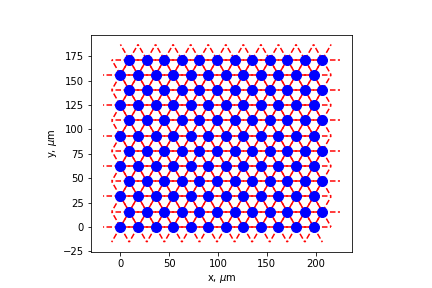
\includegraphics[width=.9\textwidth]{assets/theory-2019-09-05-115736205-2a1.png}
  \caption{Carpet geometry as a graph: nodes are cilia, connections depict interactions}
 % \label{fig:label:3224}
\end{subfigure}
\begin{subfigure}[h]{.55\textwidth}
  \centering
  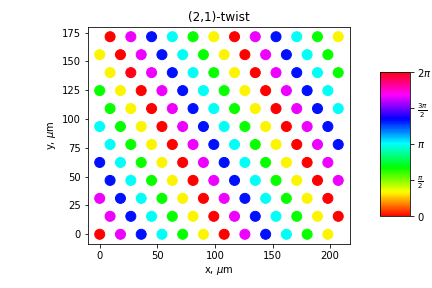
\includegraphics[width=.9\textwidth]{assets/theory-2019-09-05-120537244-7e6.png}
  \caption{Phases of cilia in $(2,1)$-twisted state}
  %\label{fig:label:323}
\end{subfigure}
\caption{}
 \label{fig:12-geom}
\end{figure}

First, we find fixed points of Poincare map $\FP_{\vec{k}}$. 

Second, we study linear stability of the fixed points. We perturb fixed points by $N-1$ perturbations of the form $\Delta_0 = \delta_0 \sin(\varphi_{\vec{m},j})$ and find $\Lmat$.

TODO: Connect to the section with L and eigenvalues

TODO: explain mapping to dual lattice space; minimum and maximum of eigenvalue importance; also dual lattice in 2D confusion: get\_k vs get\_k\_naive

TODO: continuous eigenspectrum

\subsection{Stability domains}

\begin{figure}[h]
    \centering
    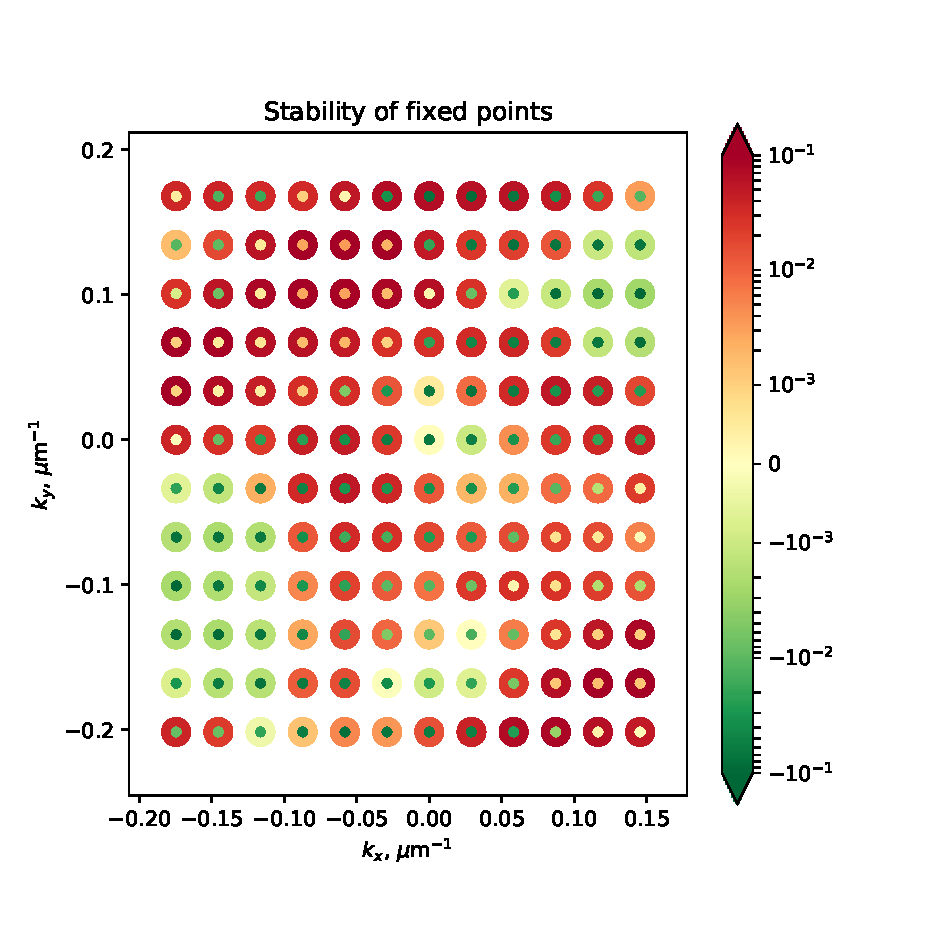
\includegraphics[width=.6\textwidth]{assets/theory-2019-09-05-124002319-236.eps}
    \caption{Linear stability of the fixed points: minimum and maximum of real parts of eigenvalues are shown in inner and outer circles. Location of the circle represents location of the fixed point in the dual lattice space. There are 3 domains of stability (domains of green circles).}
    %\label{fig:crack}
\end{figure}

\begin{figure}[h]
    \centering
    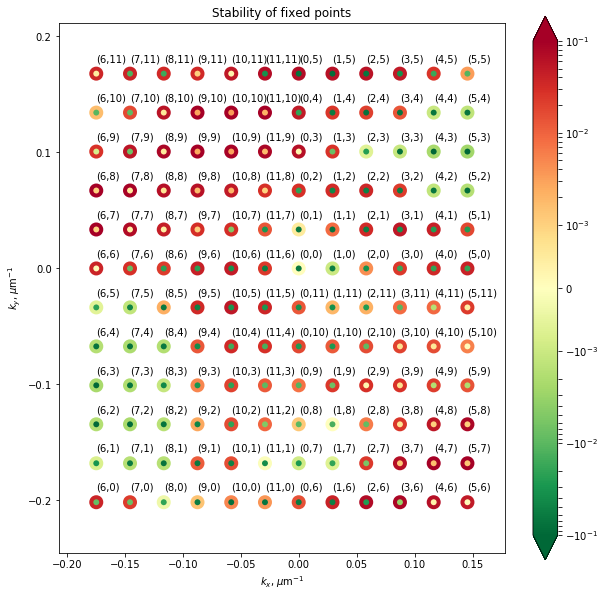
\includegraphics[width=.6\textwidth]{assets/m-twist-map.png}
    \caption{To understand how wave numbers $k_1$ and $k_2$ correspond to the wave vector $\vec{k}$}
    %\label{fig:crack}
\end{figure}

\subsection{Eigenspectrum}
Let's consider a fixed point $\FP_{\vec{k}}$, its Lyapunov exponents and eigenvectors $\lambda_j$,$\D_j$, We can map each eigenvector to a complex exponent of an $\vec{m}$-twist\eqref{eqn:delta_to_k}:
\begin{equation}
\D_j = \eps \exp(i\F_{\vec{m}_j}),
\label{eqn:delta_to_m}
\end{equation}
here we keep small number $\eps$ as a reminder that only small perturbations are allowed in linear regime.

\begin{figure}[h]
\begin{subfigure}[h]{.55\textwidth}
  \centering
 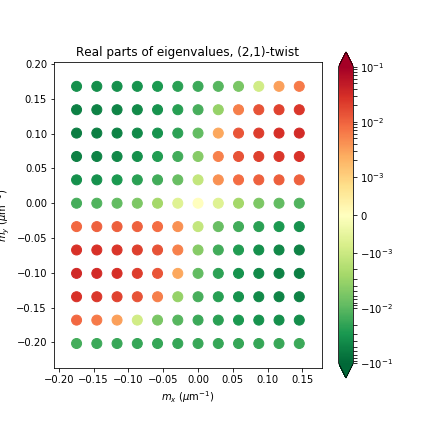
\includegraphics[width=.9\textwidth]{assets/theory-2019-09-05-163844330-50c.png}
  \caption{$(2,1)$--twist}
 % \label{fig:label:3224}
\end{subfigure}
\begin{subfigure}[h]{.55\textwidth}
  \centering
  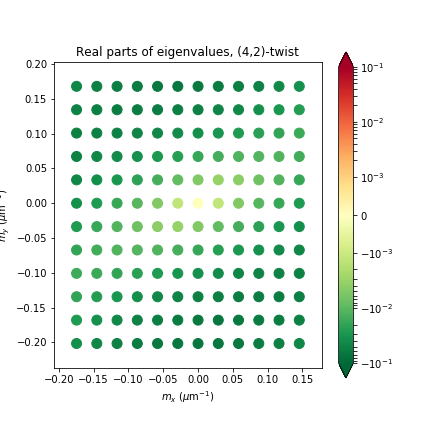
\includegraphics[width=.9\textwidth]{assets/theory-2019-09-05-163949584-d0f.png}
  \caption{$(4,2)$--twist}
  %\label{fig:label:323}
\end{subfigure}
\caption{Real parts of eigenvalues, as a function of $\vec{m}$}
 %\label{fig:12_geom}
\end{figure}

Period of oscillations is slightly different at each of the limit cycles (Fig. \ref{fig:period})

TODO: explain how I group it.

\begin{figure}[h]
    \centering
    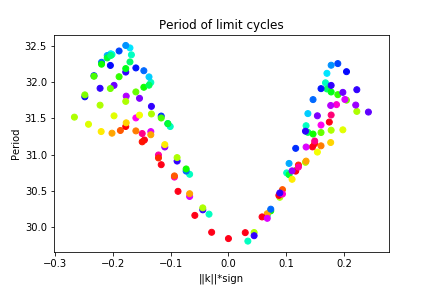
\includegraphics[width=.6\textwidth]{assets/period.png}
    \caption{Period of limit cycles, depending on $\vec{k}$, $x$-axis shows $\vec{k}$ length, color denotes angle $\theta$ from $0$ to $\pi$, points which have angle $\theta +\pi$ have the same color, but negative position on $x$-axis.}
    \label{fig:period}
\end{figure}



\clearpage
\section{Toy model: chain of oscillators with trigonometrical coupling}
% Command for this section
\newcommand*{\fr}[2]{\frac{2 \pi #1} {N} #2 } %shortcut for 2pi k / N * j
\newcommand*{\si}[2]{\sin  \fr{#1}{#2} } %shortcut for sin, cos, exp(2pi k / N * j x)
\newcommand*{\co}[2]{\cos \fr{#1}{#2} } 
\newcommand*{\ex}[2]{e ^{i \fr{#1}{#2}}}



\begin{align*}
\dot \varphi_j = \omega_0 + \sum_{n,m} ( & s_{nm}\sin(m\phi_j - n \phi_{j-1}) + s_{nm}\sin(m\phi_j - n \phi_{j+1}) +\\
+ & c_{nm} \cos(m\phi_j - n \phi_{j-1}) + c_{nm} \cos(m\phi_j - n \phi_{j+1}) ), \quad j=1..N
\end{align*}

\begin{itemize}
\item If there no non-zero terms with $n \neq m$, pure m-twists will be limit cycles. Frequency will be modified by cosine terms.
\end{itemize}



\subsection{Sine coupling }
\textit{Jupyter notebook try14b
}
Similarly looking eigenvalues and stability regions \cite{zou2009}
\subsubsection{Formulation}

Consider a chain of $N$ oscillators with equal beating frequency $\omega_0$, simple sinusoidal coupling and periodic boundary conditions (below we consider index $j$ modulo $N$).

\begin{equation}
\dot \varphi_j = \omega_0 (
1 + \lambda_s \sin(\varphi_j - \varphi_{j-1})
+ \lambda_s \sin(\varphi_j - \varphi_{j+1})), \quad j=1..N
\label{eqn:dphidt-sine}
\end{equation}

Limit cycles are perfect m-twists with some wave number $k$

$$
\varphi_j(t) = \omega_0 t - \fr{k}{j}, \quad j=1..N
$$
Indeed, if we substitute that into \eqref{eqn:dphidt-sine} we find that for  $\forall j$ $\dot \varphi_j = \omega_0$.

From our simulations we guess that eigenvectors will be a sine or cosine of an m-twist with some wave number $m$.

To prove it, let's perturb the limit cycle and find how this perturbation will develop in time
$$
\varphi_j \big\rvert_{t=0} = - \fr{k}{j} + \eps \exp( - i \fr{m}{j}), \quad j=1..N
$$
\textit{
Note that calculations don't change if we perturb with only $\cos$ or $\sin$ of an m-twist. General form is necessary when we add cosine coupling terms.
}

\subsubsection{Derivation}

Substitute that into \eqref{eqn:dphidt-sine} - see scanned pdf notes \textit{[and see appendix; references via latex gives only an empty link]}

\begin{equation}
\dot \varphi_j \big\rvert_{t=0} = 
\omega_0 \left( 1 +  2 \lambda_s  \co{k}{} \left(1 - \co{m}{} \right) \eps \exp( - i \fr{m}{j}) \right)  
+ \bigO(\lambda_s \eps ^2 \omega_0)
\end{equation}

Let's rewrite it in an abstract form

\begin{equation}
 \varphi_j = -  \fr{k}{j}  + \eps  v_j \implies 
\dot \varphi_j =  \omega_0 + A \eps  v_j + \bigO(\lambda_s \eps ^2 \omega_0)
\label{eqn:dphidt-sin-abstract}
\end{equation}

where $v_j =\exp( - i \fr{m}{j})$, $A$ - a constant. Note that this relation doesn't change if we add any constant (independent of $j$) to $\varphi_j$. The relation holds for any small $\eps$, so let's modify $\eps$ by time-dependent factor $\alpha(t)$, assuming $\alpha(t) = \bigO(1)$

\begin{equation}
\varphi_j(t) = -  \fr{k}{j} + \omega_0 t + \alpha(t) \eps v_j, \quad \alpha(0) = 1
\label{eqn:phi-sin-ansatz2}
\end{equation}

Then the derivative relation \eqref{eqn:dphidt-sin-abstract} becomes

\begin{equation}
\dot \varphi_j  = \omega_0 + A \eps \alpha(t)  v_j + \bigO(\lambda_s \eps ^2  \omega_0)
\end{equation}

Substituting \eqref{eqn:phi-sin-ansatz2} to the left-side and omitting higher order terms on the right side, we obtain an ODE for $\alpha(t)$

\begin{equation}
\omega_0 + \dot \alpha \eps v_j  = \omega_0  + A \eps \alpha(t)  v_j 
\end{equation}

\begin{equation}
\dot \alpha  = A \alpha(t), \quad \alpha(0) = 1
\end{equation}

The solution is an exponential function
\begin{equation}
\alpha(t) = e^{A t}
\end{equation}
and 
\begin{equation}
\varphi_j(t)  =  -  \fr{k}{j} + \omega_0 t +  e^{A t}  \eps v_j.
\quad t = \bigO(\Re(A)^{-1})
\end{equation}

Therefore we found how phases evolve in time after a perturbation in a vicinity of a limit cycle, and showed that $v_j$ are indeed components of an eigenvector. 
In case of $\Re(A) > 0$ this solution is valid only on time scales of $\bigO(\Re(A)^{-1})$, otherwise $\alpha = \bigO(1)$ is not satisfied.

After one oscillation cycle at time $T$ perturbation strength changes by factor $e^{AT}$, therefore
\begin{equation}
\varphi_j(T) - \varphi_j(0) = (e^{AT} - 1) v_j
\end{equation}
This mean that linearized Poincare map eigenvalue \textit{(Floquet multiplier)}
$$
\Lambda = e^{A T}
$$
Eigenvalue of the logarithm of linearized Poincare map \textit{(dimensionless form of Lyapunov eigenvalue)}
$$
\lambda = \ln \Lambda = A T
$$
This relation with A is expected, as the coupling strength doesn't depend on phase (only on phase difference).

\subsubsection{Results}

The perturbation grows or decays with exponential rate $A$ (Lyapunov exponent)
$$
A = 2 \lambda_s \omega_0 \co{k}{} \left(1 - \co{m}{} \right)
$$

Since eigenvalues are real, we can construct purely real eigenvectors. These are $\eps \si{m}{j}$ and  $\eps \co{m}{j}$: N linear-independent eigenvectors.

Oscillation frequency is unmodified in the presence of coupling. Period $T = \frac{2 \pi}{\omega_0}$.


Poincare map eigenvalue
$$
\lambda = 4 \pi \lambda_s  \co{k}{} \left(1 - \co{m}{} \right)
$$
Floquet multiplier 
\footnote{
In case of sufficiently weak coupling we can write
$$
\Lambda 
= 4 \pi \lambda_s  \co{k}{} \left(1 - \co{m}{} \right) - 1  + \bigO(\lambda_s^2),
$$
but in practice to be safe we should stick to a general formula, as the difference is notable already at $\lambda_s = 0.01$.
}
$$
\Lambda = \exp \left( 4  \pi \lambda_s  \co{k}{} \left(1 - \co{m}{} \right) \right)
$$



\subsubsection{Conclusions. Visualizations}
\begin{itemize}
\item Fixed points (limit cycles) are pure m-twists.
\item All eigenvalues (and eigenvectors) are real.
\item Frequency is unchanged
\item All eigenvalues are degenerate with degeneracy = 2, except for $m=0$, $m=N / 2$ (if N is even).
\item At any fixed point, all eigenvalues are either non-negative, or non-positive.
\item Eigenvalues at $k=\pm\frac{N}{4}$  are all zero.
\item Checked the difference between simulation and analytical calculations: only higher order terms remain, as predicted by analysis.

\end{itemize}

The perturbation decays if $\Re(A)$ is negative. The limit cycle is stable if for any perturbation $A$, or equivalently $\lambda$ are negative (more precisely - non-positive, since we always have a neutral perturbation).


Visualize eigenvalues at $N=12$, $\lambda_s = - 0.01$. 


\begin{figure}[h]
    \centering
    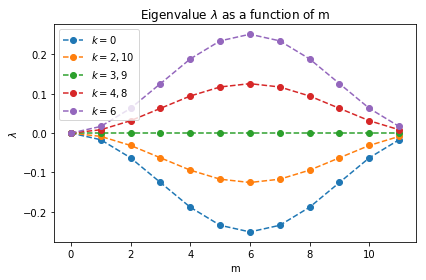
\includegraphics[width=.6\textwidth]{assets/theory-2019-08-27-181128169-abc.png}
    % \caption{}
    %\label{fig:crack}
\end{figure}

\begin{figure}[h]
    \centering
    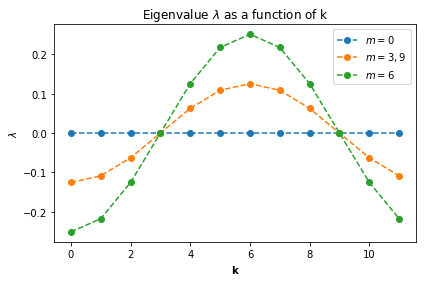
\includegraphics[width=.6\textwidth]{assets/theory-2019-08-27-181132121-3da.png}
    % \caption{}
    %\label{fig:crack}
\end{figure}


\clearpage

\subsection{Sine plus cosine coupling}
\textit{[try14c]}

\subsubsection{Formulation}


\begin{equation}
\dot \varphi_j = \omega_0 \left( 
1 
+ \lambda_s \sin(\varphi_j - \varphi_{j-1})
+ \lambda_s \sin(\varphi_j - \varphi_{j+1})
+ \lambda_c \cos(\varphi_j - \varphi_{j-1})
+ \lambda_c \cos(\varphi_j - \varphi_{j+1}) \right)
\label{eqn:dphidt-sin-cos}
\end{equation}

Let's consider a complex perturbation

$$
\varphi_j \big\rvert_{t=0} = - \fr{k}{j} + \eps \exp( - i \fr{m}{j})
$$

\subsubsection{Derivation}

Again substitute into derivative [see pdf notes 2019-08] and end up with

$$
\dot \varphi_j = \omega + A \eps \exp(- i \fr{m}{j}) + \bigO(\lambda_0 \eps ^ 2 \omega_0),
$$
where 

$\lambda_0 = \bigO(\lambda_s, \lambda_c)$, e.g. $\lambda_0 = \left( \lambda_s^2 + \lambda_c^2 \right)^{\frac{1}{2}}$ - measure of coupling strength,


\subsubsection{Results}

$\omega$ - effective frequency\footnote{Higher order terms scaling as $\eps ^2$ confirmed in simulation}
$$
 \omega = \omega_0 (1 + \lambda_c \co{k}{}) + \bigO(\lambda_0 \eps^2 \omega_0 ),
$$

$A$ - perturbation change rate --- Lyapunov exponent

$$ 
A = 
 2 \lambda_s \omega_0 \co{k}{} \left(1 - \co{m}{} \right)
- 2 i \lambda_c \omega_0 \si{k}{} \si{m}{},
$$

Eigenvalue of logarithm of linearized Poincare map \textit{(dimensionless Lyapunov exponent)} $\lambda = A T$, where $T = \frac{2 \pi}{\omega}$
$$
\lambda
=\frac{4 \pi} {1 + \lambda_c \co{k}{}} \left(  \lambda_s \co{k}{} \left(1 - \co{m}{} \right)
-  i \lambda_c \si{k}{} \si{m}{} \right) 
$$
Floquet multiplier
$$ 
\Lambda = e^{\lambda}
$$

\subsubsection{Conclusions. Visualizations}

\begin{itemize}
\item Fixed points (limit cycles) are pure m-twists.
\item Frequency depends on cosine coupling strength, and phase difference at the limit cycle.
\item Now eigenvalues and eigenvectors are in general complex, degeneracy is broken (but not always: $k=\pm \frac{N}{4}$).
\item Lyapunov exponent at $k=\pm\frac{N}{4}$  is purely imaginary, degeneracy = 2.
\item At any fixed point, all Lyapunov exponents have either all non-negative, or all non-positive real parts.
\item Contributions from sine and cosine coupling terms are additive in Lyapunov exponent, but not in dimensionless one, and especially not in Poincare map eigenvalue, unless $\lambda_0$ is sufficiently small. 
\item Checked the difference between simulation and analytical calculations: only higher order terms remain, as predicted by analysis.
\end{itemize}

\textbf{Visualize eigenvalues} at 
$\lambda_s = - 0.01$, $\lambda_c = 0.01$, $N=12$.

Lyapunov/Poincare exponents $\lambda$ and Floquet multipliers $\Lambda$ change similarly with $m$, but not exactly in the same way. Lyapunov exponents which have the same imaginary part, but different real time evolve in time differently, and therefore Poincare map eigenvalues have slightly different imaginary parts.

\begin{figure}[h]
    \centering
    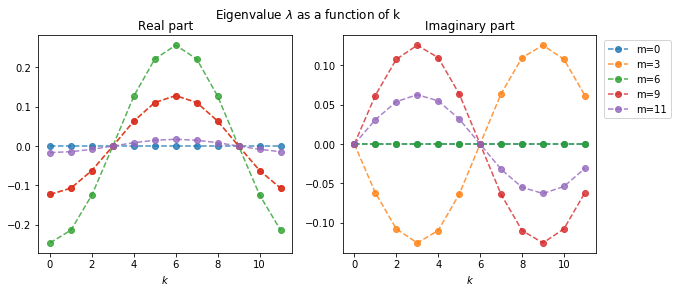
\includegraphics[width=.95\textwidth]{assets/theory-2019-09-06-173919422-458.png}
    % \caption{}
    %\label{fig:crack}
\end{figure}


\begin{figure}[h]
    \centering
    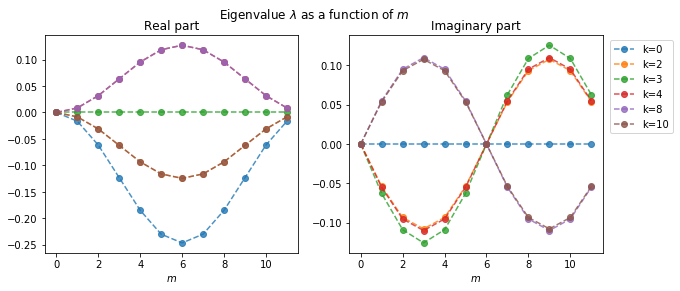
\includegraphics[width=.95\textwidth]{assets/theory-2019-08-27-181719526-a8d.png}
    % \caption{}
    %\label{fig:crack}
\end{figure}

\begin{figure}[h]
    \centering
    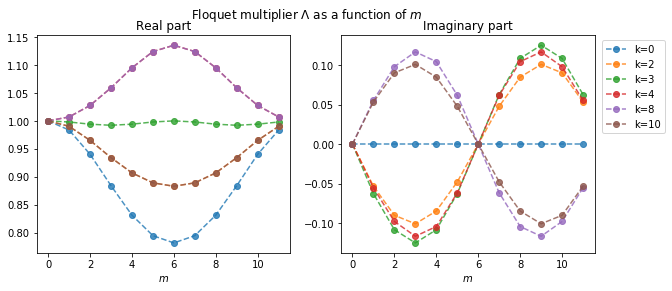
\includegraphics[width=.95\textwidth]{assets/theory-2019-08-27-181703429-803.png}
    % \caption{}
    %\label{fig:crack}
\end{figure}

\begin{figure}[h]
    \centering
    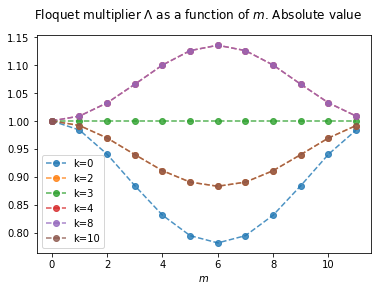
\includegraphics[width=.55\textwidth]{assets/theory-2019-08-27-182315374-a22.png}
    % \caption{}
    %\label{fig:crack}
\end{figure}

\clearpage

\begin{appendices}
\section{Numerical inaccuracy discussion}


\subsection{Inaccuracy in fixpoint}

\subsubsection{Fixpoint}


\begin{itshape}
{\small 
Ben suggested a different notation:
\begin{itemize}
\item  difference between real fixpoint and approximate: $\wt \D_0$
\item  After one cycle distance to the real fixpoint: $\wt \D_1$
\item Then always use $\D_0$, $\D_1$ like before

\end{itemize}
Downsides:

\begin{itemize}
\item New $\wt \D_1$ is not $\D_*$, but we can only compute latter.
\item In code we subtract numerical fixpoint, but we should  subtract its Poincare map image.
\end{itemize}

}
\end{itshape}

We find fixpoint by optimization procedure [defined above] up to a tolerance, specified in code. Two tolerances are involved: (i) solver tolerance and (ii) minimizer tolerance. After some minimal testing, those were taken to be equal and further in this section both are referred simply as tolerance.

Suppose we found numerically a fixpoint $\wt \Phi^*$, but it is not perfect and $ \mathcal{L}(\wt \FP) \neq \wt \FP $:

$$ \mathcal{L}(\wt \FP) = \wt \FP + \D_*$$

This means, that real fixpoint is somewhere else:

$$\wt \FP= \FP + \wt{\D}$$

If we consider linear approximation in vicinity of $\FP$


$$ \mathcal{L}(\wt \FP) = \FP + \mathbf{L}  \wt{\D}$$

$$ \wt \FP + \D_* = \FP + \mathbf{L}  \wt{\D}$$

$$  \FP + \wt{\D} + \D_* = \FP + \mathbf{L}  \wt{\D}$$

Therefore

\begin{equation}
\D_* = ( \mathbf{L} - \mathbf{I} ) \wt{\D} + \mathcal{O}(\lVert \wt{\D} \rVert^2)
\label{eqn:delta-star}
\end{equation}



Note
\begin{itemize}

\item We don't know real $\mathbf{L}$ (only approximate at $\wt \FP$)
\item We don't know distance to the real fixpoint $\wt{\D}$.
\item We can, however, calculate $\D_*$.

\end{itemize}

Let's denote
 $\varepsilon_{F}
 = \lVert \D_* \rVert
 =\lVert \mathcal{L}(\wt{\FP}) - \wt{\FP}  \rVert$
and $\delta_F = \lVert \wt{\D} \rVert $. Then

$$
\lVert \D_* \rVert = \lVert ( \mathbf{L} - \mathbf{I} ) \wt{\D} \rVert
$$


$$
\min|\lambda| \delta_F
\leq \varepsilon_{F}
\leq \max|\lambda| \delta_F
$$

$$
\varepsilon_{F} \sim |\lambda| \delta_F
$$



\subsubsection{Perturbed state}
Let's consider a perturbed (approximate) fixpoint. Fixpoint error will add up to the perturbation:

$$
\mathcal{L}(\wt{\Phi}^* + \D_0)
= \mathcal{L}(\FP + \wt  \D +  \D_0 )
= \FP +  \mathbf{L}  ( \wt{\D} +  \D_0 )
$$
The left side is equal to the initial state plus deviation

$$
\mathcal{L}(\wt \FP  + \D_0)
= \wt \FP + \D_1
= \FP + \wt{\D}  + \D_1
$$

And combining these two equalities

$$
\D_1
=  \mathbf{L}   \D_0  + (\mathbf{L} - \mathbf{I}) \wt{\D}
$$

$$
\D_1 - \D_0
=  (\mathbf{L} - \mathbf{I})  \D_0  + (\mathbf{L} - \mathbf{I}) \wt \D
$$

$$
\D_1 - \D_0
=  (\mathbf{L} - \mathbf{I})  \D_0  + \D_*
$$

Now let's estimate norms

$$
\lVert \D_1 - \D_0 \rVert
\sim
|\lambda|(\delta_0 + \delta_F)
\sim
|\lambda|\delta_0 + \varepsilon_F
$$

$$
\frac{ \lVert \D_* \rVert }  {\lVert \D_1 - \D_0 \rVert }
\sim
\frac{ \varepsilon_F } { |\lambda| \delta_0 + \varepsilon_F}
$$

If $|\lambda| \delta_0 >>  \varepsilon_{F}:$

$$
\frac{ \lVert \D_* \rVert }  {\lVert \D_1 - \D_0 \rVert }
\sim
\frac{ \varepsilon_F } { |\lambda| \delta_0}
\sim
\frac{ \delta_F } {  \delta_0 }
$$


\paragraph*{Conclusions}
- We want to make sure that $\frac{ \lVert \D_* \rVert }  {\lVert \D_1 - \D_0 \rVert } $ is small. Otherwise, $\D_1 - \D_0$ is significantly affected by $\D_*$ contribution, and we will have big error when we calculate matrix $\mathbf{L}$. TODO: quantify

- $\D_1 - \D_0$ has a constant contribution equal to $\D_*$.
- Note that $\D_0$, $\D_1$ - simulation input and outputs, so that's something we can directly obtain.
- $ \D_* $ - is something that we can measure, and can control indirectly, by tuning
  algorithm tolerance.
- Therefore, we must make sure that
  - Test at $N=6$ showed that this ratio is around or below $10^{-2}$ if fixpoint tolerance is $10^{-8}$.

- Also, just for fun, let's note

$$
 \mathcal{L}(\wt \FP  + \D_0) - \mathcal{L}( \FP  + \D_0) = D\mathcal{L} \vert_{\wt \FP  + \D_0} \wt \D + \mathcal{O}(\delta_F^2)
$$


\subsubsection{Linearized map}
Expand Poincare map $\mathcal{L}$ in vicinity of $\FP$

$$
\mathcal{L}(\wt \FP+ \D_0)
= \FP +  \mathbf{L}  ( \wt \D +  \D_0 ) + \mathcal{O}(( \delta_F + \delta_0)^2)
$$ % = ... + \mathcal{O}(\delta_F^2, \delta_F \delta_0,  \delta_0^2)

Do the same in vicinity of $\wt \FP$

$$
\mathcal{L}(\wt \FP + \D_0)
= \mathcal{L}(\wt \FP) +  \wt{\mathbf{L}} \D_0 + \mathcal{O}(\delta_0^2) =
$$

$$
=  \FP + \Lmat \wt \D + \mathcal{O}(\delta_F^2)  +  \wt{\mathbf{L}} \D_0 + \mathcal{O}(\delta_0^2)
$$%= \FP + \wt \D + \D_* +  \wt{\mathbf{L}} \D_0 + \mathcal{O}(\delta_0^2)


Combining those two

$$
\mathbf{L}  ( \wt \D +  \D_0 ) + \mathcal{O}(( \delta_F + \delta_0)^2)
=
\Lmat \wt \D + \mathcal{O}(\delta_F^2)  +  \wt{\mathbf{L}} \D_0 + \mathcal{O}(\delta_0^2)
$$


$$
\mathbf{L} \wt \D 
=
 \wt{\mathbf{L}} \D_0 + \mathcal{O}(( \delta_F + \delta_0)^2)
$$

$$
(\mathbf{L} -  \wt{\mathbf{L}}) \D_0 
=
a_{10} \delta_0 + a_{01} \delta_F + a_{20}  \delta_0^2 + a_{02} \delta_F^2 + a_{11} \delta_0 \delta_F + ...
$$

The left side scales linearly with $\delta_0$, since it must hold for any $\delta_0$ (sufficiently small), only terms which scale linearly with $\delta_0$ can exist.

$$
(\mathbf{L} -  \wt{\mathbf{L}}) \D_0 
=
\delta_0 \bigO(\delta_F)
$$
And finally
$$
\mathbf{L} -  \wt{\mathbf{L}}
=
 \mathcal{O}(\delta_F)
$$

\textit{$\Lmap(\wt \FP)$ and $\wt \FP$ are asymptotically at the same distance from $\FP$.}

\begin{equation}
\Lmap(\wt \FP) = \FP + \Lmat \wt \D + \mathcal{O}(\delta_F ^2)
\end{equation}
Or
\begin{equation}
\Lmap(\wt \FP) - \FP = \bigO((1 + |\lambda|) \delta_F) = \bigO(|\lambda|)
\end{equation}
\subsubsection{Numerical estimations}

If $N = 6$, fixpoint with $ tol  =10 ^{-8}$:

$|\lambda| = 10 ^ {-2}$ - $10 ^ {-3}$

$\varepsilon_F = 10 ^ {-6}$ - $10^{-7}$

Therefore $\delta_F \sim 10 ^{ -4}$

If $\delta_0 = 10 ^{-3}$, $\frac{ \delta_F } {  \delta_0 } = 10^{-1}$, and indeed,
$ \frac{ \lVert \D_* \rVert }  {\lVert \D_1 - \D_0 \rVert }$ lie in range $2 * 10^{-2} - 10 ^{-3} $



\section{Analytical derivation of eigenvalues for a chain of oscillators with sinusoidal and cosinusoidal coupling} 
\includepdf[pages=-]{2019-08-28-sin-cos-eigenspectrum.pdf} 

\end{appendices}


\clearpage

\bibliographystyle{apsrev4-1}%  https://journals.aps.org/revtex/revtex-faq
%AMA style gives errors
\bibliography{carpet2}

\end{document}

